\newcommand{\CLASSINPUTtoptextmargin}{0.75in}
\newcommand{\CLASSINPUTbottomtextmargin}{1in}
\newcommand{\CLASSINPUToutersidemargin}{0.75in}
\documentclass[10pt,twocolumn]{IEEEtran}

\usepackage[pdftex]{graphicx}

\begin{document}
\title{Mitigation of Industrial Control System Attacks Using A Boosted Filter Ensemble}

\author{\IEEEauthorblockN{Kelvin Ly\IEEEauthorrefmark{1}, Jacob Hazelbaker\IEEEauthorrefmark{1}, Andrew Hughes\IEEEauthorrefmark{1}, Orlando Arias\IEEEauthorrefmark{1} \\Faculty Advisor: Yier Jin\IEEEauthorrefmark{2}}\\
\IEEEauthorblockA{\IEEEauthorrefmark{1}{Department of Electrical and Computer Engineering, University of Central Florida}}\\
\IEEEauthorblockA{\IEEEauthorrefmark{2}{Department of Electrical and Computer Engineering, University of Florida}}\\
{rangertime@knights.ucf.edu, oarias@knights.ucf.edu, yier.jin@ece.ufl.edu}\vspace{-0.16in}\vspace{-0.2in}}

\maketitle
\pagestyle{empty}
\thispagestyle{empty}

\begin{abstract}
Aging and legacy control systems suffer from an increasingly urgent threat from cyberattacks.
However, it is often difficult, expensive, or impossible to upgrade these legacy systems to reduce the threat of attack.
Thus, it makes more sense to develop defense modules that can be added to these legacy systems to improve their resilence under the threat of cyberattack.

We develop a control system testing framework as well as a defense module that relies on a robust attack detection algorithm.
The testing framework may be used to test both attacks and defenses on control systems, and is integrated with Simulink to allow for ease of use and integration into existing design workflows.
The framework is designed to be extensible and to work with any programmable logic controller that provides a Modbus TCP slave interface, potentially allowing testing on the hardware that could be used in production.

The defense module acts as a wrapper for the programmable logic controllers, exposing a Modbus TCP slave interface that the control system is connected to.
The attack detection algorithm uses a diverse ensemble of machine learning algorithms, each of which is independently trying to detect unusual activity from both the sensor data and the actuator commands from the PLCs.
These different methods are combined together using gradient boosting to produce a highly robust filter.
\end{abstract}

\section{Introduction}
The CSAW 2017 Embedded Security Challenge focuses on security industrial control systems against attacks on programmable logic controllers (PLCs) and sensors.
The challenge is based around the problem of securing a system built on top of legacy PLCs.
These PLCs will be running code that we will not have access to, and consequently, they effectively act as black boxes that may or may not be controlled by the attacker.
Similarly, the sensors may or may not be compromised by the attacker.
Following Shannon's maxim, we assume the attacker has an almost perfect knowledge of the system, in terms of its implementation, aside from not knowing some set of secrets.
The goal overall is to deploy a system on top of the existing infrastructure to mitigate an attacker's ability to cause the system to break by allowing it to enter an unsafe state.

Control systems offer an unusual attack surface compared to other modern systems.
The use of legacy communications systems often means that control system must be air gapped to prevent attackers from hijacking the unencrypted and sometimes unauthenticated communication between the control center and the controllers.
For example, the Modbus standard, one of the most commonly used standards for PLC to SCADA communications, lacks authentication or authorization features \cite{modbus}.
The PLCs themselves differ greatly between manufacturers, with each manufacturer including their own vendor-specific extensions functions to IEC 61131-3, the standard that specifies five languages that PLC programs can be written in.
Many of the PLCs expose different administrative panels, some of which are known to have vulnerabilities \cite{metasploit}.
Some approaches to secure PLCs through introducing hardened MCUs or improved protocols run into the fact that such changes would be unlikely to be accepted by industry, as they would mean costly and risky replacements of important parts of their systems.
Consequently, our attempt to defend PLCs tries not to make too many assumptions about the low-level properties of the devices, treating them as black boxes that may or may not be functioning correctly.

There are two different forms of attacks, attacks that alter the output of the PLCs, and attacks that alter the outputs of sensors in the system.
Our defense against both of these consists of providing predictors that try to predict the future state of the system, estimators that support the predictors by estimating unknown hidden variables, and classifiers that use the predictions and estimations to determine whether a given deviation should be classified as an attack or failure.
The predictors and estimators here will be a combination of some of the ones commonly found in control theory and those used in machine learning.
This ensemble of classifiers will be combined together using gradient boosting to provide a hopefully robust single classifier that can accurately detect attacks.
Apart from sharing this basic framework, PLC outputs and sensor outputs will also have some additional security measures that take advantage of their individual attributes.

Overall, our contributions are:
\begin{itemize}
\item A testing framework tightly integrated with MATLAB Simulink to allow testing of control systems for robustness and resilience under attack.
\item A (hopefully) robust algorithm for detecting attacks using a combination of many individual classifiers.
  This will be efficient enough to run on a Raspberry Pi without affecting its ability to also act as a PLC.
\end{itemize}

This paper will first discuss the current state of the art in control system defense, then it will discuss the process through which the defense module was developed, followed by details of the system's implementation, some further discussion of the design, and then the conclusion.

\section{Related Works} \label{sec:related}
False data injection detection is very much still an open research area.
A lot of work has been done in it for the specific case of large power grid systems, beginning with the work by Yao which demonstrated that a family of attacks were possible which were undetectable from normal power grid operation from the standpoint of state estimation \cite{liu2011false}.
Various other papers devised methods to overcome this shortcoming, such as by choosing a small subset of sensors that could be protected to prevent false data injection attacks \cite{bobba2010detecting}.

Cardenas et al noted that defenses in control systems tended to focus on generating a handful of carefully designed metrics, each of which would attempt to detect one particular type of failure mode for the system \cite{attacks}.
This meant that the system was only secure if every failure mode was accounted for, leaving room for human error, especially given how the complexity of control systems often means different components can interact in complicated ways that would not at all be straightforward to predict.
The publication advises the development of more robust attack-detection algorithms, as well as building attack tolerance into the control systems themselves.
They focus their defense on defending against integrity attacks, their name for attacks that alter sensor data.
They define three different types of stealthy attacks, surge attacks (where the attacker attempts to do as much damage without being detected as soon as they gain access to the system), bias attacks (where the attacker adds a small constant to the value of their compromised sensor), and geometric attacks (where the attacker causes their compromised sensor to drift exponentially away from its correct value).

Fawzi et al develop a general approach to building attack-resiliant control systems \cite{secureestimation}.
In order to do this they develop a robust state estimation algorithm that could provide a best estimate of the real state of the system that was inspired by error correction algorithms.
They then show how such a state estimation can be translated into control system stabilization, and thus the state estimation algorithm developed in the first part of the publication can be the basis of a robust control system, assuming some sort of feedback occurs within the control system.
The formal model they use closely matches that used in this paper.
They assume that an attacker controlled a small number of sensors and controllers within the system, and that the attacker can arbitrarily alter the values generated in the places they control.
However, they make the further assumption that the control system can be represented exactly as a linear system, which differs from this paper, where it is considered to be a black box.
The state estimation uses an error correcting step, which uses the linearity of the system to solve for and correct a finite number of errors by using data collected from a finite number of time steps of the system.

Mishra et al examine state estimation for control systems under attack by a static adversary in the presence of Gaussian measurement noise \cite{noise}.
They follow a similar argument as Fawzi et al, assuming the control system is linear, and perform a brute force search over all the sensor subsets to determine the set that most likely matches reality.
They prove that their approach provides optimal protection against attacks, and then extend their results to nonlinear systems to show it that a similar approach is possible there.

Shoukry et al employ a vastly different approach to more efficiently solve for the system state estimate than in previous works \cite{modulo}.
They note that previous approaches either did not provide complete protection, or suffered from an explosion in time complexity because they try to enumerate every potential combination of uncompromised sensors.
Their approach solves the problem by using a combination of a SAT solver and a theory solver to determine the sensors that are more likely to be under attack and then calculating the current system state based on that knowledge.
The SAT solver tries to guess which sensors are under attack, and then the theory solver acts to provide further constraints to avoid contradictions when the SAT solver guesses wrong.
The authors prove that this system is both guaranteed to terminate under some fairly loose conditions, and then further optimize it to improve execution time.
They develop some heuristics to accelerate the search for the subset of sensors that are under attack, and benchmark them to examine their performance characteristics.
Their approach proves to be substantially faster and scalable to larger numbers of sensors compared to methods in prior works.

\section{Background} \label{sec:bg}
Our approach towards this problem differs from the signal processing branch, where it becomes an optimal control theory problem, and from cybersecurity, where it becomes a network security problem.
We attempt to frame the problem as a machine learning classification problem, trying to distinguish signals originating in normal operation from those originating in compromised devices.
Nothing else is assumed of the signals other than that some of them will be attempting to maintain their particular values near their respective setpoints.
The largest problems faced with this approach are that the signals will probably not vary too greatly from the setpoint, making it hard to collect useful data to prevent machine learning algorithms from overfitting, and that there is comparatively little data being collected during online operation for the machine learning algorithms to learn from.

Consequently, it seems sensible to use a diverse set of machine learning algorithms to improve the chances of one or more of them working for a specific control system.
This would hopefully mean that one or more of the algorithms chosen will perform well for a given system, and then could be used as the primary classifiers for that system.
This step of the process can be performed using adaptive boosting, a meta algorithm that is known to perform well and to be more resistant to overfitting than other algorithms \cite{adaboost}.

\section{Implementation} \label{sec:impl}
\begin{figure*}
  \centering
  
\includegraphics[width=0.7\textwidth]{csaw2017architecture.png}
  \caption{High level overview of the test framework}
  \label{fig:arch}
\end{figure*}

The project can be separated into a testing framework integrating MATLAB that allows control systems built in Simulink to be used as test platforms, and the actual protection system used to detect and warn about potential attacks on the simulated control system.
The overall architecture can be seen in Figure \ref{fig:arch}.
In a real life use case, essentially everything could be stripped out of the system except for the defense module, which would act as it does now as a proxy between the control system and the PLCs.

\subsection{Test Framework} \label{sec:test}
The control system is simulated using MATLAB on a separate computer using Simulink.
The PLC is connected using a set of Simulink blocks created during this project that can translate Simulink signals into Modbus commands.
These blocks are written in C, using MATLAB's S-block functionality, and use \texttt{libmodbus} to communicate using Modbus TCP.
Each block keeps track of real time as well as simulation time, so that they can ensure the simulation stays in time with real world time.
All communication past this point is done using Modbus TCP.

MATLAB's Simulink PLC Coder was used to generate IEC61131-3 Structured Text function blocks, which were fed into a code generator that produces structured text code that would simulate a set of simulated PLCs.
This code generation parses the function block to extract its input and output variables, and then generates a complete structured text program with the function block instantiated multiple times.
The code generator also had to make some modifications to the function block, because OpenPLC does not appear to support the same set of features as those used by the PLC Coder.
Namely, PLC Coder generates constant variables, which are not recognized by OpenPLC's structured text compiler.
The code generator has to do some rudimentary constant folding to circumvent this; it acts as a preprocessor and replaces all instances of the constant variable name with its value.
It then maps holding registers and coils to all the function blocks' inputs and outputs, making them accessible from Modbus TCP and consequently from Simulink.

\begin{figure}
  \centering
  
\includegraphics[width=\columnwidth]{csaw2017sensorwrite.png}
  \caption{Communication done during a sensor write request}
  \label{fig:write}
\end{figure}

\begin{figure*}
  \centering
  
\includegraphics[width=0.7\textwidth]{csaw2017plcread.png}
  \caption{Communication done during a PLC output read request}
  \label{fig:read}
\end{figure*}


A stack of Modbus proxies, with OpenPLC's Modbus TCP slave endpoint at the bottom, provides the combination of attack simulation and defense testing.
The Simulink blocks communicate with the top of the stack, which then forwards the request down in the stack, while potentially altering the request or response, as can be seen in Figures \ref{fig:write} and \ref{fig:read}.
In this way, the first attack proxy can alter sensor input by modifying sensor data write requests it receives from MATLAB.
This allows attacks that modify the sensor inputs to the PLCs to be simulated.

After this first proxy is the defense module.
During sensor write data requests the defense module duplicates the sensor data so that each simulated PLC will receive its sensor data, and also keeps a sample of the sensor data for attack detection.
When the control system tries to read the PLC output, the defense module duplicates that request as well, but modifies the response so that the control system receives whatever response it deems correct.
The exact details of this module will be discussed further in this paper.

The defense module proxies requests to the other attack module, which simulates attacks on PLCs.
In this attack module, the responses from the PLC are altered during PLC output read requests.
This module then communicates directly to the OpenPLC Modbus TCP slave, completing the connection between the Simulink system and the PLC logic.

\begin{figure}
  \centering
  
\includegraphics[width=\columnwidth]{csaw2017workflow.png}
  \caption{Workflow for model testing}
  \label{fig:workflow}
\end{figure}

A lot of the complexity in this system is primarily meant to make it possible to use existing tools and knowledge to build the control systems that are to be tested.
The overall process can be seen in Figure \ref{fig:workflow}.
The first step in preparing a system for testing is to either create or find a Simulink model for it.
This model is then used to generate the PLC code, and then it is also slightly modified to allow it to function with the rest of the test framework.
This is a fairly simple procedure, and thus testing PLC security using this framework could potentially be easily integrated into existing engineering design workflows fairly easily.

\subsection{Defense Module} \label{sec:def}
Our method builds on top of the current standard for using redundancy to improve system reliability, enhancing it to be more robust.
Our system should be able to withstand some attacks where the attacker controls a majority of the controllers, and can detect some attacks on the sensors within the system as well.
In an attempt to provide a robust, general solution that can reliably detect a large number of attacks than simple majority voting cannot.
The system will use an ensemble of approaches to determine the likelihood of error or attack originating from any of the PLCs.
These of these approaches will individually calculate the likelihood of a failing or compromised PLC.
These approaches will include modeling the PLCs as time delay neural networks, hidden Markov models, and low order control systems, using simple majority voting, and classifying their behavior using support vector machines.
After some experimentation, some of the lower scoring approaches may be pruned to improve the performance of the system.

\subsubsection{Security mechanisms exclusive to PLCs}
Only one, if any, of the PLCs, will be virtually connected to the plant at any moment.
All the PLCs will receive sensor data for each time step, but only the output of one of them will actually be fed into the actuators in the system.
If the system predicts that an attacker has assumed complete control over all the PLCs, the system will temporarily switch into running using the predictors and estimators described above.
Their control over the actuators will be time multiplexed, with the length of each PLC's time slot governed by the classifiers' belief in that given PLC's trustworthiness, preventing any attacker from exerting too much control over the system.

Additionally, the devices which are not at a given instant controlling the plant may be subject to various disturbances, which will provide additional data that can be used to characterize the PLCs.
In particular, this will prevent some of the machine learning algorithms from overfitting by broadening the conditions they observe.
It is expected that the systems are probably naturally fairly stable, and consequently most of the data collected will be of the system working at or near its set point.
Emulating disturbances allows a more complex model that more accurately predicts system behavior to be developed.

\subsubsection{Filters to be implemented}
This section will cover the different systems that will feed into the gradient boosting algorithm.
Each of these will independently model, predict, and monitor the inputs and outputs of PLCs and sensors.

One filter will be a simple majority filter.
Given an odd number of redundant PLCs, the filter will select the median value of the PLCs.
The standard deviation of the output will be measured online, and this estimate will be continually improved as the system runs.
Any PLCs deviating from the median value past a certain multiple of the standard deviation will be marked as faulty.

Another filter will be use least means square to estimate the control system, and each PLC using third order models.
The filter will constantly accept new data to improve its estimates, and it will also maintain some confidence value for the accuracy of the parameters.
A PLC whose parameters deviate noticeably from those of the others, or whose signal violates its own predicted signal by a noticeable margin, will be marked as faulty.

A third filter will attempt to use time delay neural networks to model the system, PLCs, and sensors.
It will attempt to classify the signal at any moment as belonging either within stable operation, or as belonging to a compromised or failed device.

\subsection{Test Models}\label{sec:models}
Two models have been modified to work for this project.
The first one was a model of a coffee making plant, and the second was the fairly well known Tennessee Eastman acrylic plant model.

\begin{figure*}
  \centering
  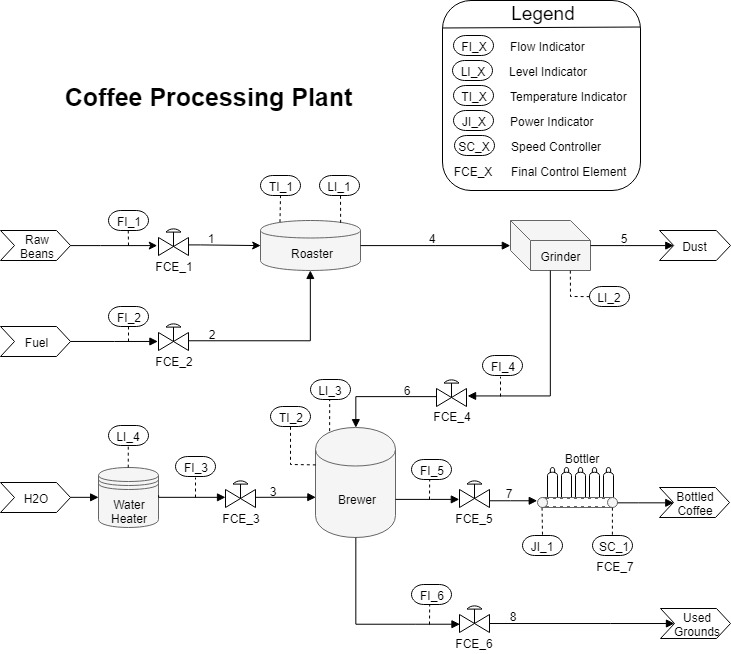
\includegraphics[width=0.8\textwidth]{coffee.png}
  \caption{Block diagram for the coffee plant}
  \label{fig:coffee}
\end{figure*}

\begin{figure*}
  \centering
  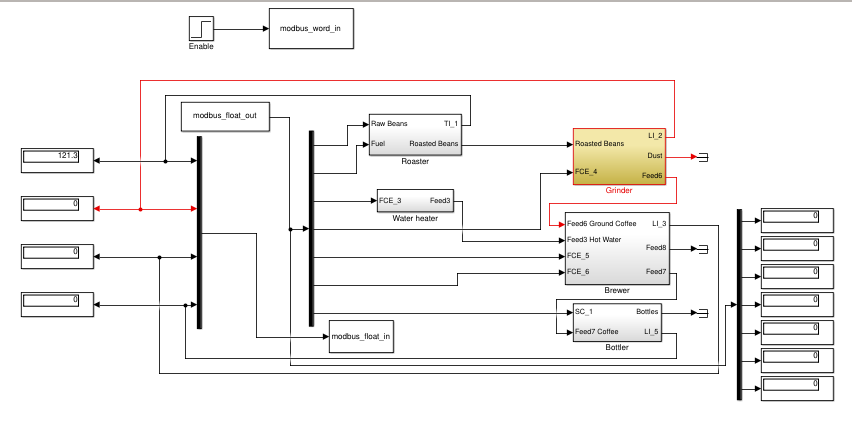
\includegraphics[width=\textwidth]{coffee_simulink.png}
  \caption{Simulink model of the coffee plant for testing}
  \label{fig:coffee_simulink}
\end{figure*}

The first model was created specifically for this project (block diagram is in Figure \ref{fig:coffee} and Simulink model is in Figure \ref{fig:coffee_simulink}).
Although it is meant to model the process involved in creating bottles of brewed coffee, the structure should be similar to other industrial plants where some reaction takes place between two reactants within some temperature range, along with some preprocessing of both of the reactants.
It also have the distinction of not being covered by the methods mentioned in the related works; those methods assumed a linear control equation, whereas this system uses bang-bang control, which is still used in systems where the precision and expense of precisely controlled actuators are not needed.
The model includes assertions within the subsystems, so that the model will stop with an error if any invalid conditions occur.
These errors include any of the various tanks overflowing or underflowing, or the coffee roaster not reaching the desired temperature range before coffee beans are added.

The Tennessee Eastman model is a model of a chemical plant that been a popular choice in control systems papers \cite{te0,te1,te2,te3,te4}.
This system is modelled after a real life chemical plant with a large assortment of reactors, sensors, actuators, using flow rates and reaction rates.
Consequently, it has proven effective in demonstrating the practicality of various control system theories.
Several Simulink models of the system already existed, so one of those was chosen to use in this project.
A recent, modernized revision of the model was used, which luckily had all of the control logic clearly and neatly separated from the system model \cite{te_revised}.

\section{Discussions}\label{sec:discussion}
This system uses many separate, fairly robust, well studied algorithms as a result of the very general nature of the problem it is attempting to solve.
Industrial control systems are very diverse, and consequently any attempt to protect them in a general case must be very robust to adequately work in a large number of systems.
It isn't expected that any one of these algorithms can adequately model all control systems, but it is expected that at least some of them will perform well enough for all control systems.
The gradient boosting performed acts to select the set of algorithms that work well for each system.

\section{Neural Network Defense Security Analysis}\label{sec:future}
One very promising alternative approach towards control system security would be to use a variation of generative adversarial networks to potentially discover and learn new possible attacks much more quickly than the previous set up.
In the canonical generational adversarial network setup, one algorithm is learning to forge something, while the other algorithm is learning how to distinguish forgeries from the real product \cite{gan}.
The objective in that case was to train the generative model to produce articles that are nearly indistinguishable from the real thing, whereas in this case there would be a few subtle changes to use the same basic idea to develop a model that can detect increasingly deceptive attacks, as well as a model that develops increasingly stealthy attacks.
This would be done by adjusting the algorithm slightly.
Thus, instead of attempting to just fool the defense module, the generative model would also be scored on how effective the attacks that went undetected were.
Some score, such as the total amount the state variables of the system deviated from their setpoints, could be used here.
The defense module would be given a sample of data from both sensors and the PLC outputs, and would try to determine whether this was from normal operation or from some type of attack.
Over time, the generative model should learn how to generate more sophisticated data modifications to try to fool the defense module, and the defense module should learn how to deal with more covert attacks\footnote{Note that we are still working on the adversarial neural network defense and the implementation may not be demonstrated during the on-site demonstration session.}.

%This idea was discovered fairly late in the process, and thus was not completed by the deadline for this paper. This may or may not be finished by the time of the competition.

\section{Demonstration} \label{sec:conclusion}
Live demonstrations will be presented during the on-site phase at CSAW ESC 2017. We welcome judges to stop by our site for more details of our implementations. 


\vspace{-0.08in}
\raggedright
\bibliographystyle{IEEEtran}
\bibliography{mybiblio}

\end{document}
